\documentclass[12pt,letterpaper,titlepage]{article}
\usepackage[latin1]{inputenc}
\usepackage{amsmath}
\usepackage{amsfonts}
\usepackage{amssymb}
\usepackage{tikz}
\usepackage{pgf}
\usetikzlibrary{arrows,automata}
\author{Dimitri Demergis \\ Jason Lee \\ Stephen Lombardi \\ Marcus McCurdy}
\title{CS544 Group 5 Protocol}
\begin{document}
\maketitle

\section{Introduction}

\section{Services}

\section{Messages}
\begin{itemize}
\item SessionRequestMessage This message is sent by the client to the server. It is used to notify the server that it should provision a new streaming session. It also includes
the version numbers of the protocol the client supports.
\item SessionMessage This is the servers reply to the SessionRequestMessage. It tells the client what version of the protocol that will be used during the streaming session. It
also contains the session id that will be used in further communication with the server.
\item StreamMessage These messages are sent while the protocol is in the streaming state. They contain the actual data that is being streamed.
\end{itemize}
\section{DFA}
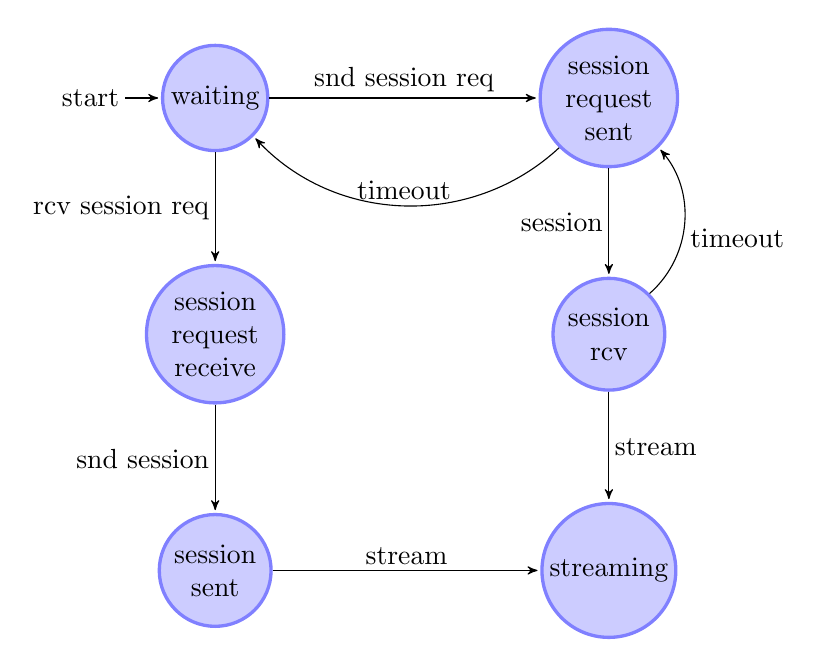
\begin{tikzpicture}[->,align=center,>=stealth',shorten >=1pt,auto,node distance=3cm,bend angle=45,inner sep=2pt, every state/.style={draw=blue!50,very thick,fill=blue!20}]
\node[initial,state] (waiting) {waiting};
\node[state, node distance=5cm] (session req sent) [right of=waiting] {session \\ request \\ sent};
\node[state] (session request receive) [below of=waiting]{session \\ request \\ receive};
\node[state] (ready) [below of=session request receive]{ready};
\node[state] (version sent) [below of=session request receive]{session \\ sent};
\node[state] (session receive) [below of=session req sent]{session \\ rcv};
\node[state] (streaming) [below of=session receive]{streaming};


\path (waiting) 		edge				node 			{snd session req} (session req sent)
	   					edge				node[swap] 		{rcv session req} (session request receive)
	(session req sent) 	edge [bend left]	node[swap] 		{timeout} 	(waiting)
						edge				node[swap]		{session} (session receive)
	(session request receive)		edge				node[swap]		{snd session}	(version sent)
	(session receive)		edge				node			{stream} (streaming)
						edge [bend right]	node[swap]		{timeout} (session req sent)
	(version sent)		edge				node			{stream} (streaming)
					
	;

\end{tikzpicture}

\end{document}